\section{АЛГОРИТМІЧНЕ ЗАБЕЗПЕЧЕННЯ ПРОЦЕСУ СТВОРЕННЯ КОРПОРАТИВНОЇ СИСТЕМИ}

\subsection{Проектування системи}
На початку розробки будь-якого програмного продукту слід значну увагу приділити проектуванню системи, адже саме від цього буде залежати легкість і правильність подальшої розробки системи, її підтримка і удосконалення.
Саме тому проектування визначає основну складову програмного забезпечення. 
Необхідні пункти для успішного запуску  продукту:
\begin{itemize}
	\item побудова UML діаграми класів;
	\item побудова діаграми відношень між об'єктами;
	\item проектування бази даних;
	\item створення макетів майбутнього інтерфейсу;
	\item чітке розмежування модулів системи і їх взаємодія і тому подібне.
\end{itemize}

\par Як було згадано вище, перш за все слід розробити діаграму класів, показати всі взаємовідношення між об'єктами, їх роль у системі та загальну взаємодію.
\subsubsection{Модель архітектури системи}
Вся робота системи організована за принципом MVC шаблону.
\par Модель-вид-контролер -- архітектурний шаблон, який використовується під час проектування та розробки програмного забезпечення.
\par Як показано на рисунку \ref{pic:mvc} цей шаблон поділяє систему на три частини: модель даних, вигляд даних та керування. Застосовується для відокремлення даних (модель) від інтерфейсу користувача (вигляду) так, щоб зміни інтерфейсу користувача мінімально впливали на роботу з даними, а зміни в моделі даних могли здійснюватися без змін інтерфейсу користувача.

\par Головна мета використання даного шаблону -- гнучкий дизайн програмного забезпечення, який повинен полегшувати подальші зміни чи розширення програм, а також надавати можливість повторного використання окремих компонент програми. 
Крім того використання цього шаблону у великих системах призводить до певної впорядкованості їх структури і робить їх зрозумілішими завдяки зменшенню складності.

\begin{figure}[!ht]
\centering
		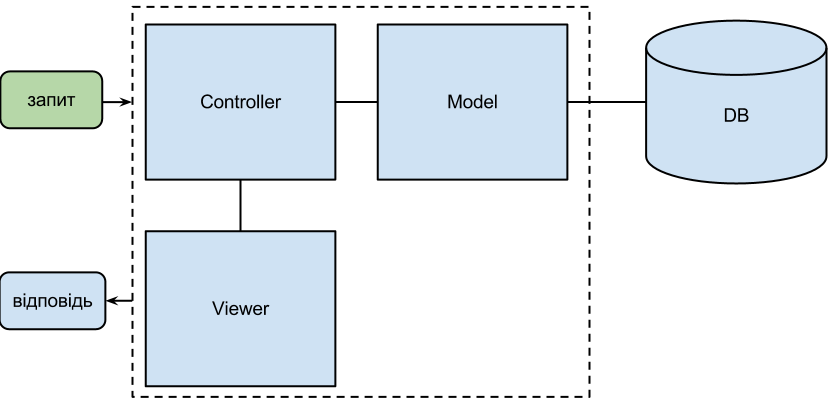
\includegraphics[width=1.00\textwidth]{mvc.png}
		\vspace{18pt}
		\captionof{figure}{Архітектура MVC}\label{pic:mvc}
\end{figure}

\par Як згадувалося раніше, архітектурний шаблон Модель-Вид-Контролер (MVC) поділяє програму на три частини. У тріаді до обов'язків компоненту Модель (Model) входить зберігання даних і забезпечення інтерфейсу до них. Вигляд (View) відповідальний за представлення цих даних користувачеві. Контролер (Controller) керує компонентами, отримує сигнали у вигляді реакції на дії користувача і повідомляє про зміни компоненту Модель. Така внутрішня структура в цілому поділяє систему на самостійні частини і розподіляє відповідальність між різними компонентами.
\par MVC поділяє цю частину системи на три самостійні частини: введення даних, компонент обробки даних і виведення інформації. Модель, як вже було відмічено, інкапсулює ядро даних і основний функціонал з їх обробки. Також компонента Модель не залежить від процесу введення або виведення даних. Компонента виводу Вигляд може мати декілька взаємопов'язаних областей, наприклад, різні таблиці і поля форм, в яких відображається інформація. У функції Контролера входить моніторинг за подіями, що виникають в результаті дій користувача (зміна положення курсора миші, натиснення кнопки або введення даних в текстове поле).
Зареєстровані події транслюються в різні запити, що спрямовуються компоненті Моделі або об'єктам, відповідальним за відображення даних. Відокремлення моделі від вигляду даних дозволяє незалежно використовувати різні компоненти для відображення інформації. Таким чином, якщо користувач через Контролер внесе зміни до Моделі даних, то інформація, подана одним або декількома візуальними компонентами, буде автоматично відкоригована відповідно до змін, що відбулися.


\subsection{Проектування бази даних}
База даних базується на СКБД MySQL -- відкритій системі. Взаємозв'язок із користувачами відбувається через Модель системи (див. рис. \ref{pic:mvc}). В базі містяться всі необхідні дані. Паролі користувачів зберігаються у шифрованому вигляді.
\par Реляційна система керування базами даних (РСКБД; інакше Система керування реляційними базами даних) -- СКБД, що керує реляційними базами даних.
\par Поняття реляційний (англ. relation -- відношення) пов'язане з розробками відомого англійського спеціаліста в області систем баз даних Едгара Кодда (Edgar Codd).
\par Ця модель характеризується простотою структури даних, зручним для користувача табличним представленням і можливістю використання формального апарату алгебри відношень і реляційного обчислення для обробки даних.
\par Реляційна модель орієнтована на організацію у вигляді двовимірних таблиць. Кожна реляційна таблиця являє собою двовимірний масив і має такі властивості:
\begin{itemize}
	\item кожний елемент таблиці -- один елемент даних;
	\item всі комірки в стовпці таблиці однорідні, тобто всі елементи в стовпці мають однаковий тип;
	\item кожний стовпець має унікальне ім'я;
	\item однакові рядки в таблиці відсутні;
	\item порядок наступності рядків і стовпців може бути довільним.
\end{itemize}
Базовими поняттями реляційних СКБД є:
\begin{itemize}
	\item атрибут;
	\item відношення;
	\item кортеж.
\end{itemize}

\subsubsection{InnoDB механізм}
\par InnoDB це потужний механізм (рушій) для зберігання даних, розроблений фінською компанією Innobase Oy, яка була придбана в 2006 році концерном Oracle Corporation.
\par Поширюється за ліцензією GNU General Public License. Є у всіх нових версіях MySQL, і, починаючи з версії 5.5 для MySQL механізм за замовчуванням.
\par Застосування InnoDB дозволяє використання базою даних таких функцій, як транзакції, зовнішні ключі. Він також сумісний з ACID.
\par У цьому рушії є два способи для зберігання даних: файл або група файлів, загальних для всіх баз даних і таблиць, або один файл даних для кожної таблиці. Інші важливі особливості InnoDB: блокування на рівні рядків, можливість стиснення даних і MVCC.

\subsubsection{Відношення в таблицях}
\par Головною одиницею бази даних є таблиця яка відповідає за дані користувачів, адже саме від неї залежать більшість таблиць. Для прикладу це повідомлення, чи завдання.
\par Для зв'язку між таблицями використовуються зовнішні ключі. Зовнішній ключ -- це атрибут (набір атрибутів) в деякому відношенні R, який відповідає первинному ключу іншого відношення або того ж таки відношення R.
\par Ці взаємозв'язки представляються у вигляді відношень. Розділяють три види відношень:
\begin{itemize}
	\item Багато-до-багато (n:m);
	\item Один-до-багато (1:m);
	\item Один-до-одного (1:1).
\end{itemize}
\par Багато-до-багатьох SQL відносин використовується, коли деяка невизначена кількість рядків (n) в таблиці пов'язані з невизначеною кількістю рядків (m), які зберігаються в іншій таблиці. Це називається: (m:m) відносини, тому що (n) рядків у першій таблиці, відносяться до (m) рядків в іншій.
\par Потрібно бути впевненим, що використовується кількість рядків строго більше ніж одиниця, тому що у випадку із одиницею слід використовувати відношення один-до-багатьох (1:n).
\par Розглянемо приклад, який зберігає країни в одну таблицю і мови в іншу таблицю. Є країни в світі, де більш ніж одна офіційний мова, і відповідно є випадки коли говорять одною мовою більш ніж в одній країні. Саме для цього призначене відношення багато-до-багатьох. 
\par Приклад створення такої бази даних продемонстрований нище:
\lstinputlisting[language=SQL]{code/one-to-many.sql}

\par Реалізація такої структури таблиць зображено на рисунку \ref{pic:many_to_many.png}.
\begin{figure}[!ht]
\centering
		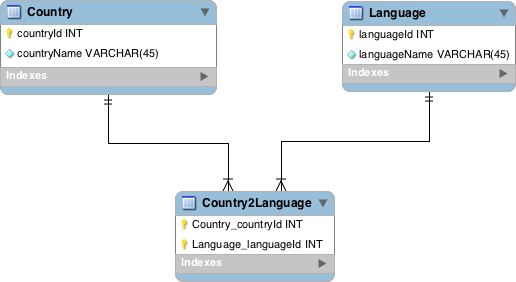
\includegraphics[scale=0.8]{many-to-many.png}
		\vspace{18pt}
		\captionof{figure}{Відношення багато-до-багато}\label{pic:many_to_many.png}
\end{figure}

\par Один-до-багато (1:n) відношення є дуже поширеним в SQL. Основна ідея полягає в тому, що кожен рядок зберігається в одній таблиці та пов'язаний з невизначеною кількістю рядків у іншій таблиці. Це може бути будь-яке число між 0 і (n) рядків.
\par Дуже хорошим прикладом є SQL база даних, яка зберігає замовлення в одній таблиці (перша частина) і порядок позицій в іншій (n-на сторона). Приклад такої структури таблиць зображено на рисунку \ref{pic:one_to_many.png}.
\begin{figure}[!ht]
\centering
		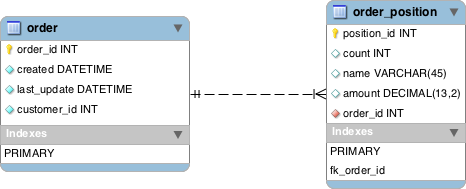
\includegraphics[scale=0.8]{one-to-many.png}
		\vspace{18pt}
		\captionof{figure}{Відношення один-до-багато}\label{pic:one_to_many.png}
\end{figure}
\par Реалізувати відношення один-до-багатьох дуже просто. Відносини зберігаються за допомогою спеціальної колонки в n-таблиці. Ця колонка містить один первинний ключ. Якщо присутні ще первинні ключі, то просто потрібно додати ще декілька стовпців.

\par У наведеному вище прикладі, потрібно додати до основної колонки таблиці <<order>> (поле <<order\_id>>) позицію в таблицю <<order\_position>>. Саме для того щоб забезпечити цілісність даних, використовуються зовнішні ключі.
\par Основною перевагою один-до-багатьох є доступність нормалізації таблиць і при цьому не потрібно нагромаджувати таблицю непотрібними даними.


\par Один-до-одного відношення в SQL використовують для того щоб розділити великі таблиці на менші при цьому без втрат продуктивності. В деяких випадках це краще ніж величезна EAV \cite{EAV} таблиця. 
\par Ідеальний варіант використання відносин 1:1 для не пов'язаних зв'язків, які поділяють основні ознаки, як для прикладу каталог записів. Приклад такої структури таблиць зображено на рисунку \ref{pic:one_to_one.png}.
\begin{figure}[!ht]
\centering
		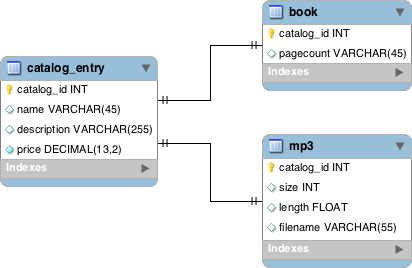
\includegraphics[scale=0.8]{one-to-one.png}
		\vspace{18pt}
		\captionof{figure}{Відношення один-до-одного}\label{pic:one_to_one.png}
\end{figure}
\par Ідея цієї концепції полягає в тому, що таблиця, яка містить основні атрибути, які є загальними для всіх суб'єктів. У першому каталозі загальні атрибути містять назву продукту, опис і ціну для прикладу. А самі атрибути, які є специфічними для певних видів продукції зберігаються в окремих таблицях. Зв'язок між цими таблицями зберігається за допомогою тих же первинних ключів в кожній таблиці.
\par Як ви можете бачити в наведеному вище прикладі, один-до-одного може бути реалізовано за допомогою простого використання тих же первинних ключів для таблиці. 
\par Крім того, можливо використовувати різні первинні ключі і додавати відносини кожній колонці таблиці, але цей підхід має свої недоліки: SQL буде досить складним і заплутаним, і якщо використовувати зовнішні ключі, то це призведе до кругової залежності.
\par Первинний ключ -- атрибут, або набір атрибутів, що однозначно ідентифікує кортеж даного відношення. Первинний ключ обов'язково унікальний, він єдиний і найголовніший із унікальних ключів.
В реляційних базах даних первинний ключ задається обмеженням PRIMARY KEY. Для прикладу:
\begin{lstlisting}[language=SQL]
CREATE TABLE users(id INTEGER PRIMARY KEY AUTO_INCREMENT, name CHAR(20), surname CHAR(40));
\end{lstlisting}


\subsubsection{Архітектура бази даних}
Як згадувалося вище майже все базується на відношенні до таблиці користувачів. Відношення повинні базуватися на основі моделі один-до-багатьох. Загальна модель бази даних зображена на рисунку \ref{pic:db_shema}.
	
\par Як показано на рисунку \ref{pic:db_shema} -- всі таблиці у базі даних взаємозв'язані. На таблицю користувачів посилаються таблиці документів, коментарів, блогів, календарів, команд, регіонів, типу робіт, вікі, завдань та повідомлень. 
Це в свою чергу дає змогу забезпечити відношення користувача до певної категорії. 
Для прикладу один користувач може мати декілька документів чи коментарів, звідси і слідує використання відношення один-до-багатьох. 
\par Також допоміжні таблиці як категорія документів, кімнати, категорія вікі та категорія завдань мають свої відношення на головні таблиці (для прикладу одна категорія завдань може містити багато завдань).

\subsection{Зовнішній макет сайту}
Основою для користувача є зовнішній вигляд - UI (user interface) інтерфейс користувача. 
Інтерфейс користувача -- сукупність засобів для обробки та відображення інформації, максимально пристосованих для зручності користувача. У графічних системах інтерфейс користувача реалізовується багатовіконним режимом, змінами кольору, розміру, видимості (прозорість, напівпрозорість, невидимість) вікон, їхнім розташуванням, сортуванням елементів вікон, гнучкими налаштовуваннями як самих вікон, так і окремих їхніх елементів (файли, папки, ярлики, шрифти тощо), доступністю багатокористувацьких налаштувань.

\par Кінцевому користувачу не завжди цікаво що відбувається всередині програми -- тому розробляють макет майбутнього проекту, в нашому випадку -- це макет веб інтерфейсу. 

	\begin{center}
		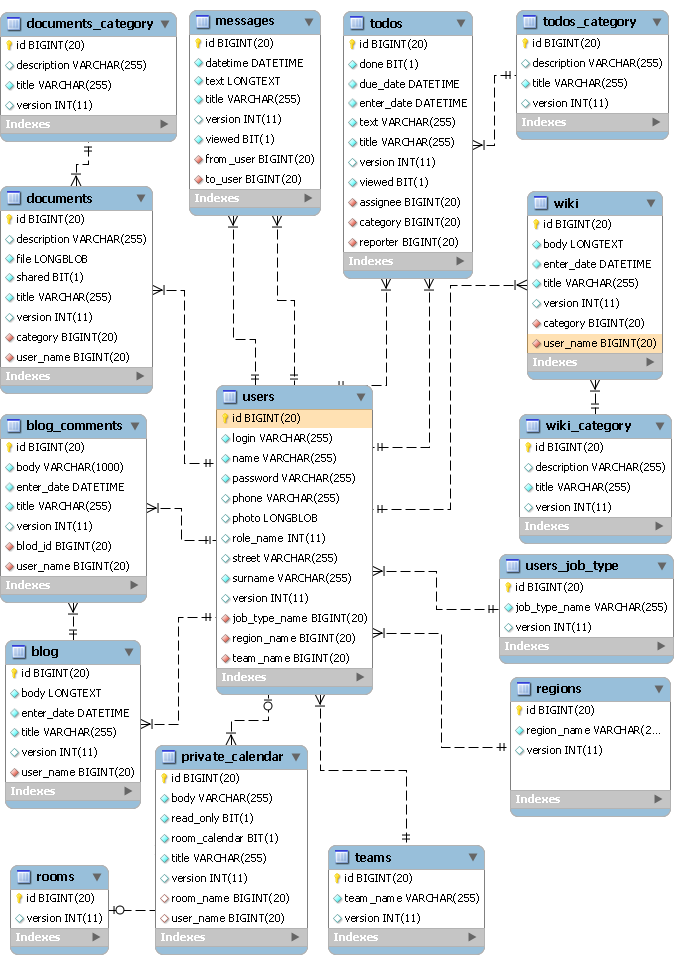
\includegraphics[width=1.00\textwidth]{db_schema.png}
		\captionof{figure}{Загальна схема структури бази даних}\label{pic:db_shema}
	\end{center}

\par Макет інтерфейсу будується в звичайному графічному редакторі. Головною метою даної розробки є максимальне відображення всіх графічних властивостей майбутнього робочого веб-сайту. Макет майбутнього сайту, зокрема головної сторінки зображено на рисунку \ref{pic:mockup}.


\begin{figure}[!ht]
\centering
		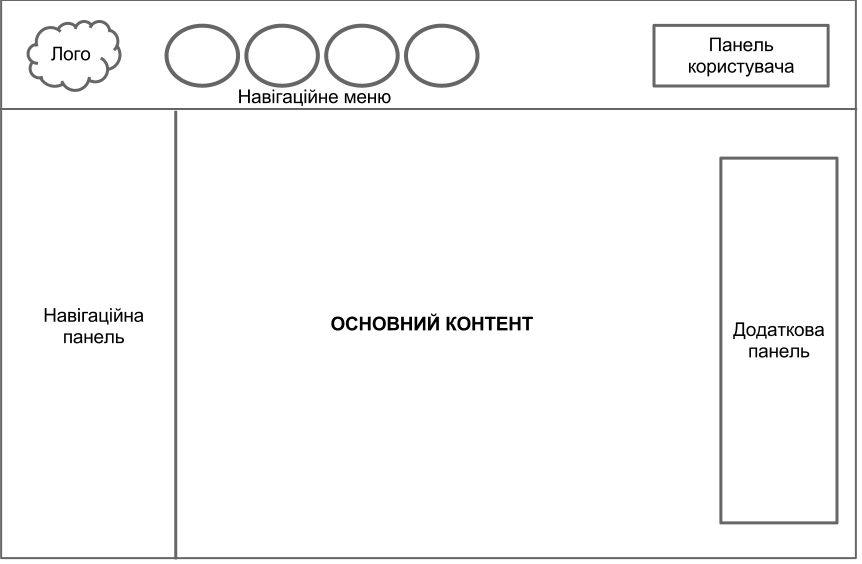
\includegraphics[width=1.00\textwidth]{mockup_mainpage.png}
		\vspace{18pt}
		\captionof{figure}{Макет майбутнього сайту}\label{pic:mockup}
\end{figure}

\par З рисунку \ref{pic:mockup}, де зображено макет сайту добре видно, що навігаційне меню розміщено зверху сайту. Дане меню повинно бути завжди доступне користувачу, тому воно завжди буде рухатися, тобто при будь якому положенні сторінки, не важливо чи внизу чи на верху, ця панель буде завжди присутня і рухатиметься за користувачем. На ній варто розмістити швидкі навігаційні кнопки, такі як: швидке створення завдання чи нотатки.
\par Зліва від всього розміщено навігаційну панель. Саме на цій панелі розміщуються всі доступні  користувачеві на веб-проекті пункти навігації. В залежності від того де в даний момент перебуває користувач, слід підсвічувати поточне меню.
\par Панель користувача розміщується справа на навігаційній панелі. Тут повинна розмістися вся інформація для керування поточним користувачем: вихід із сайту, посилання на профіль користувача, приватні налаштування.

\subsection{Структура проекту}
\par Після побудови структури бази даних та загального макету сайту, слід притупити до розробки серверної частини -- загальної структури сайту. Весь проект базується на роботі Java EE та поверх фреймворку Spring.

\subsubsection{Алгоритм роботи надбудови Java Enterprise Edition -- Spring Framework}
Архітектура Spring Framework зображена на рисунку \ref{pic:spring_arch}.

	\begin{center}
			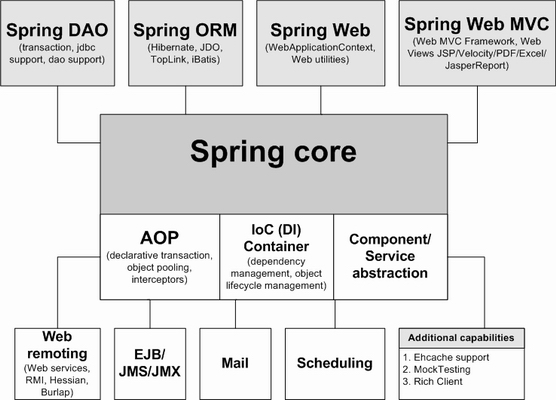
\includegraphics[width=0.80\textwidth]{spring_arch.jpg}
			\vspace{18pt}
			\captionof{figure}{Архітектура Spring Framework}\label{pic:spring_arch}
	\end{center}

\par Центральною частиною Spring Framework є Inversion of Control контейнер, який надає засоби конфігурування та управління об'єктами Java з допомогою зворотніх викликів. Контейнер відповідає за управління життєвим циклом об'єкта: створення об'єктів, виклик методів ініціалізації та конфігурування об'єктів шляхом зв'язування їх між собою.
\par Об'єкти створювані контейнером також називаються керовані об'єкти або beans. Зазвичай конфігурування контейнера здійснюється шляхом завантаження XML файлів, що містять визначення bean-ів і надають інформацію необхідну для створення bean-ів.
\par Об'єкти можуть бути отримані або за допомогою пошуку залежності, або впровадження залежності. Пошук залежності -- шаблон проектування, коли зухвалий об'єкт запитує у об'єкта-контейнера екземпляр об'єкта з певним ім'ям або певного типу. Впровадження залежності -- шаблон проектування, коли контейнер передає екземпляри об'єктів за їх іменем іншим об'єктам або за допомогою конструктора, або властивості, або фабричного методу.

\par Spring Framework містить в собі наступні програмні модулі:
\begin{itemize}
\item Inversion of Control контейнер: конфігурування компонент додатків і управління життєвим циклом Java об'єктів;
\item фреймворк аспектно-орієнтованого програмування: працює з функціональністю, яка не може бути реалізована можливостями об'єктно-орієнтованого програмування на Java без втрат;
\item фреймворк доступу до даних: працює з системами управління реляційними базами даних на Java платформі використовуючи JDBC і Object-relational mapping забезпечуючи вирішення завдань, які повторюються у великому числі Java сумічних аплікацій;
\item фреймворк управління транзакціями: координація різних API управління транзакціями і інструментарій настроюваного управління транзакціями для об'єктів Java;
\item фреймворк model-view-controller: каркас, заснований на HTTP і сервлетах, що надає безліч можливостей для розширення і налаштування (customization);
\item фреймворк віддаленого доступу: конфігурується передача Java-об'єктів через мережу в стилі RPC, підтримуюча RMI, CORBA, HTTP протоколи, включаючи web-сервіси (SOAP);
\item фреймворк аутентифікації та авторизації: конфігурується інструментарій процесів аутентифікації та авторизації, що підтримує багато популярних і стандартних протоколів, інструментів, практик через дочірній проект Spring Security (раніше відомий як Acegi);
\item фреймворк віддаленого управління: конфігурується уявлення і керування Java об'єктами для локальної або віддаленої конфігурації за допомогою JMX;
\item фреймворк роботи з повідомленнями: конфігурується реєстрація об'єктів-слухачів повідомлень для прозорої обробки повідомлень з черги повідомлень за допомогою JMS, поліпшена відправлення повідомлень за стандартом JMS API;
\item тестування: каркас, що підтримує класи для написання модульних та інтеграційних тестів.
\end{itemize}

\subsubsection{Діаграма відношень}
\par Діаграма послідовності -- в UML, діаграма послідовності котра відображає взаємодії об'єктів впорядкованих за часом. Зокрема, такі діаграми відображають задіяні об'єкти та послідовність відправлених повідомлень.
\par На діаграмі послідовностей показано у вигляді вертикальних ліній різні процеси або об'єкти, що існують водночас. Надіслані повідомлення зображуються у вигляді горизонтальних ліній, в порядку відправлення.
\par Визначені стандартом UML 2.0 діаграми послідовностей мають ті ж можливості що і визначені стандартом UML 1.x, та пітримують додаткові можливості зміни стандартного порядку повідомлень.

\par На рисунку \ref{pic:sequence} -- діаграми відношень зображено весь процес трансферу даних -- починаючи від запиту користувача, і завершуючи поверненням сформованих даних. Спочатку запит попадає на Acegi Security Controller. Після проходження перевірки користувача (детально описано в розділі \ref{sec:authority}) дані від користувача попадають на контролер, звідки всі дані для запиту передаються на модель, яка відповідає за комутацію бази даних та контролера. Після успішних проходжень цих пунктів, на контролері відбувається формування вигляду майбутньої сторінки, яка будується на базі певного виду. Після цих всіх успішних маніпуляцій, сформовані дані повертаються користувачеві, тобто на веб інтерфейс. Якщо на якомусь етапі сталася помилка, чи невірна вибірка, то кожний етап зупиняється і повертається на попередній, аж до користувача із статусом помилки.

\begin{center}
		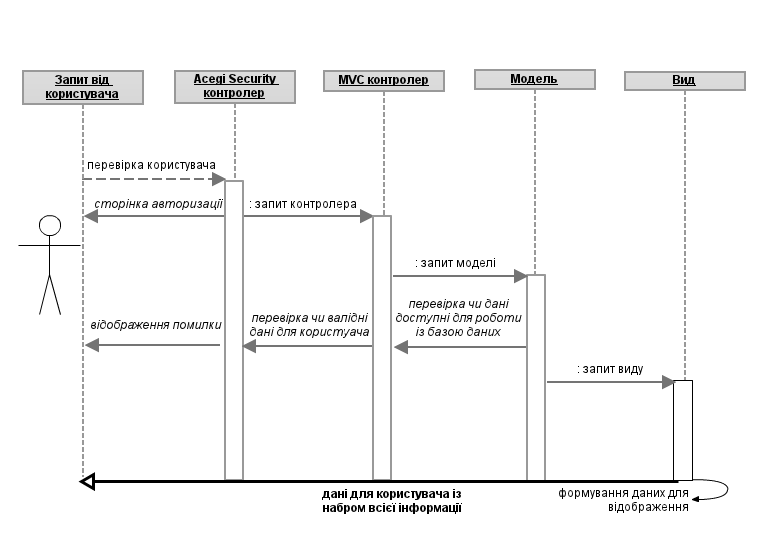
\includegraphics[width=1.00\textwidth]{sequence_diagram.png}
		\vspace{18pt}
		\captionof{figure}{Діаграма відношення запиту користувача до роботи сервера}\label{pic:sequence}
\end{center}

\subsection{Авторизація і аутентифікація}\label{sec:authority}
Основою будь-якої корпоративної системи є можливість використання системи управління користувачами.
Тому слід розробити повний цикл взаємодії користувачів. Сюди повинні бути включені наступні важливі аспекти:
\begin{itemize}
	\item можливість авторизації користувачів;
	\item ролі користувачів;
	\item зберігання даних у закодованому вигляді;
	\item чіткий розподіл прав користувачів;
	\item легка взаємодія між користувачами;
	\item можливість інтеграції із іншими сервісами системи.
\end{itemize}

\par Кожний працівник (він же користувач системи) повинний мати безперебійний доступ до свого профілю в будь-який час.
Авторизація повинна бути реалізована інтуїтивно зрозуміло для кожного користувача і легко доступна.
Управління користувачами буде реалізовано через адміністративну панель, доступ до якої будуть мати тільки користувачі певної групи.

\subsubsection{Алгоритм авторизації користувачів}
Загальний алгоритм авторизації полягає в перевірці даних користувача і повернення від серверу сформованих даних.
\par Сервер спочатку приймає надіслані від користувача логін та пароль. Логін передається на Acegi Security Controller і перекодовує пароль в шифр за допомогою алгоритму SHA-256. Адже зберігати дані не в шифрованому вигляді досить небезпечно, і у випадку, якщо зловмисник отримає їх, від цих даних не буде користі, оскільки вони шифровані і зворотнього шифру не існує. Шифрування на базі серверу відбувається через менеджер авторизації і налаштовується в конфігураційному файлі із посиланням на bean із сервісом котрий відповідає за маніпуляцію даних користувача.

\begin{lstlisting}[language=Xml]
<authentication-manager alias="authenticationManager">
	<authentication-provider user-service-ref="UserServiceBean">
		<password-encoder hash="sha-256" />
	</authentication-provider>
</authentication-manager>
<beans:bean id="UserServiceBean" class="com.diploma.ccms.service.UserService" />
\end{lstlisting}

Слід виділити наступні групи користувачів:
\begin{itemize}
	\item адміністратори;
	\item відділ кадрів;
	\item користувач без особливих прав доступу.
\end{itemize}

\par Кожній групі повинний бути забезпечений доступ до певної категорії. Це можливо реалізувати за допомогою інтрацепторів. В разі доступу користувача до недозволеної категорії, буде повернена від сервера помилка.

\begin{lstlisting}[language=Xml]
<http auto-config="true" use-expressions="true">
<form-login login-processing-url="/resources/j_spring_security_check" login-page="/login" authentication-failure-url="/login?login_error=t" />
<logout logout-url="/resources/j_spring_security_logout" />
<intercept-url pattern="/admin/**" access="hasRole('ROLE_ADMIN')" />
<intercept-url pattern="/login/**" access="permitAll" />
<intercept-url pattern="/resources/**" access="permitAll" />
<intercept-url pattern="/**" access="isAuthenticated()" />
</http>
\end{lstlisting}


\subsection{Діаграма класів}
\par Діаграма класів -- статичне представлення структури моделі. Відображає статичні (декларативні) елементи, такі як: класи, типи даних, їх зміст та відношення. Діаграма класів, також, може містити позначення для пакетів та може містити позначення для вкладених пакетів. Також, діаграма класів може містити позначення деяких елементів поведінки, однак їх динаміка розкривається в інших типах діаграм. Діаграма класів служить для представлення статичної структури моделі системи в термінології класів об'єктно-орієнтованого програмування. На цій діаграмі показують класи, інтерфейси, об'єкти й кооперації, а також їхні відносини.
\par Взаємозв'язок класу <<Команд>> і загальних інтерфейсів зображено на рисунку \ref{pic:uml}, решта класів працює за таким принципом. Кожний клас домену посилається на контролер управління та взаємозалежить від інших класів. 
Інтерфейси забезпечують уніфікації і взаємодію класів.
\begin{center}
				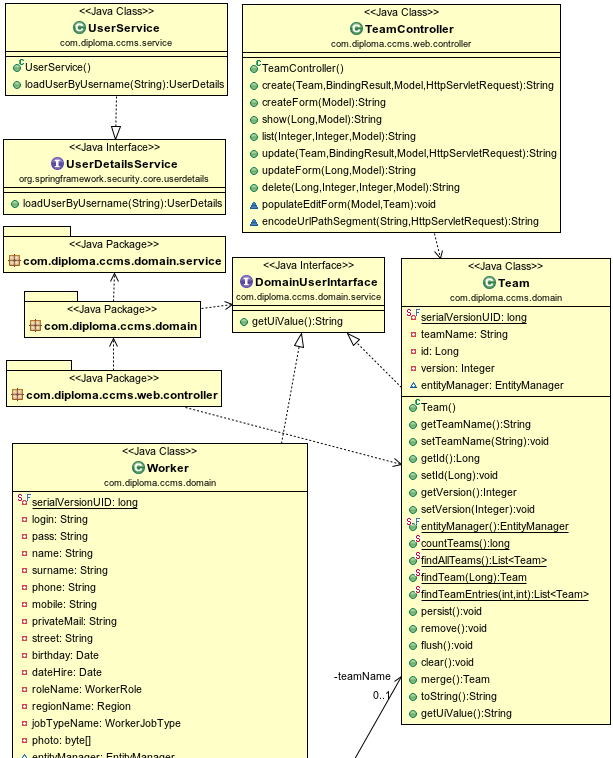
\includegraphics[width=1.00\textwidth]{uml.png}
				\vspace{8pt}
				\captionof{figure}{UML діграма взаємодії робочих до їх команд}\label{pic:uml}
		\end{center}





